\documentclass[11pt,a4paper]{article}

% ---------- Packages ----------
\usepackage[a4paper,margin=2.5cm]{geometry}
\usepackage[T1]{fontenc}
\usepackage{lmodern}
\usepackage{microtype}
\usepackage{booktabs}
\usepackage{array}
\usepackage{tabularx}
\usepackage{xltabular}
\usepackage{graphicx}
\usepackage{needspace}
\usepackage{enumitem}
\usepackage{xcolor}
\usepackage{tikz}
\usepackage{caption}
\usepackage[hidelinks]{hyperref}

\newcolumntype{Y}{>{\raggedright\arraybackslash}X}
\setlist{itemsep=2pt,topsep=4pt}
\renewcommand{\arraystretch}{1.2}
\setlength{\emergencystretch}{3em}

% ---------- Helper macros ----------
\newcommand{\cn}[1]{\texttt{#1}}   % code name (table / column)

% Data-dictionary table: \dbtable{name}{description}{rows}
\newcommand{\dbtable}[3]{%
  \Needspace{10\baselineskip}%
  \subsubsection*{\texttt{#1}}%
  #2\par\smallskip
  {\small
  \begin{tabularx}{\textwidth}{@{}>{\ttfamily}l l Y Y@{}}
    \toprule
    \textbf{Column} & \textbf{Type} & \textbf{Constraints} & \textbf{Description}\\
    \midrule
    #3
    \bottomrule
  \end{tabularx}}\par\bigskip}

% ER diagram helpers (TikZ)
% \entity{x}{y-top}{width}{height}{header-colour}{title}{attributes}
\newcommand{\entity}[7]{%
  \filldraw[thick, fill=#5] (#1,#2) rectangle ++(#3,-0.6);
  \draw[thick] (#1,#2-0.6) rectangle ++(#3,-#4+0.6);
  \node[font=\small\ttfamily\bfseries] at (#1+#3/2,#2-0.3) {#6};
  \node[anchor=north west,font=\scriptsize\ttfamily,align=left,inner sep=0pt]
        at (#1+0.15,#2-0.72) {#7};}
% horizontal relationship: \relh{x-start}{x-end}{y}{label-start}{label-end}
\newcommand{\relh}[5]{%
  \draw[thick] (#1,#3) -- (#2,#3)
     node[pos=0.2, above, font=\scriptsize] {#4}
     node[pos=0.8, above, font=\scriptsize] {#5};}

\title{waterX: Smart Plant Water Management System\\[2pt]
       \large Project Report, Requirements and Database Design}
\author{}
\date{\today}

\begin{document}
\maketitle
\tableofcontents
\bigskip

% =====================================================================
\section{Introduction}
waterX is a smart plant-water-management project with two related but
currently separate parts: a browser-based demonstration dashboard and a
Python/SQLite simulation backend. The simulator generates weather and soil
conditions, applies watering strategies and safety limits, and stores run data.
The dashboard demonstrates plant management and monitoring screens using
sample data stored in the browser; it is not connected to the simulator
database or to physical sensors.

\textbf{Research question.} Can AI-assisted watering reduce water consumption
compared with fixed-schedule watering without negatively affecting plant
growth?

This report describes the project structure, implemented behavior, known
limitations, requirements and SQLite database design. The simulator's
AI-assisted strategy currently uses a physics-based moisture forecast; a
trained machine-learning model and a measured strategy-comparison study have
not been implemented. Requirements use the MoSCoW priority scale
(\emph{Must}, \emph{Should}, \emph{Could}); implementation status is shown
separately.

% =====================================================================
\section{Project Implementation}

\subsection{Architecture and Features}
The project is organized into a Next.js frontend, a Python simulation engine
and a SQLite database. The two applications are not wired together: browser
plant and preference data is saved in \cn{localStorage}, while simulator and
seed data is saved in \cn{database/waterx.db}.

\begin{table}[htbp]
\centering
\small
\begin{tabularx}{\textwidth}{@{}l Y Y@{}}
  \toprule
  \textbf{Project area} & \textbf{Implemented features} & \textbf{Important boundary}\\
  \midrule
  Frontend & Responsive dashboard with plant-status cards, sample moisture and tank charts, sample predictions, alerts, recent watering events and quick-action dialogs. & Dashboard metrics, charts, alerts, events and recommendations are explicitly demonstration data; they are not live simulator output.\\
  Plant management & Add, edit, search, sort, filter, deactivate, reactivate and delete plants. Plant details include moisture history, watering history, growth, prediction and care settings panels. & Changes persist in this browser's \cn{localStorage}; new plants have no sensor readings.\\
  Preferences & Change the displayed profile name and light/dark appearance; reset preferences to defaults. & Preferences are local to the browser and are not user-account settings.\\
  Simulator & Hourly weather and moisture simulation; fixed-schedule, threshold-based and forecast-based watering; noisy/faulty sensor readings; tank, daily-cycle and pump-runtime safeguards; alerts and simulated growth. & The forecast is a deterministic physics-based heuristic, not a trained ML model.\\
  Database & SQLite schema, repeatable demonstration seed data, foreign-key enforcement, integrity constraints, indexes and a daily-water-usage view. & The frontend does not currently read from or write to this database.\\
  Tests & Python unit tests exercise database setup, seed repeatability, all watering strategies, data persistence, sensor/tank/pump safeguards and seeded reproducibility. & These tests do not establish frontend/backend integration or model accuracy.\\
  \bottomrule
\end{tabularx}
\caption{Implemented project components and their current boundaries.}
\end{table}

\subsection{Frontend Dashboard}
The frontend is a client-side Next.js application built with React and
TypeScript. Recharts supplies the dashboard charts, and Lucide React supplies
the interface icons. Its visual design combines a dark-blue navigation
sidebar, a top search/profile bar, a light dashboard canvas and separate
white metric and content cards. The layout reorganizes for narrower screens.
Figure~\ref{fig:dashboard} shows the dashboard design included in the project.

\begin{figure}[p]
  \centering
  \includegraphics[width=\textwidth,height=0.78\textheight,keepaspectratio]
    {\detokenize{Smart Plant Water Management Dashboard.png}}
  \caption{waterX frontend dashboard design. The cards, charts, notifications
  and recommendations are sample demonstration content, not live readings.}
  \label{fig:dashboard}
\end{figure}

\subsubsection{Dashboard overview}
The home route \cn{/} is the main monitoring screen. It presents four summary
cards for plant count and health, tank level, weekly water use and displayed
prediction accuracy. Below these cards, the plant-status section shows each
plant's category, moisture, temperature, tank level, status and next-watering
text. The right-hand activity column groups alerts and notifications, recent
watering events and quick actions. The dashboard also contains soil-moisture
trend lines with a period selector, a circular tank-level chart, a six-hour
observed-versus-predicted moisture chart, and a recommendation panel.

The top bar provides plant search, a notification button and the saved display
name. The Add Plant quick action opens a form. Other dashboard actions open
dialogs for notifications, watering history, reports, schedules or the
recommendation. The report dialog summarizes sample values; schedule editing
and database-backed reporting are not implemented.

\subsubsection{Plant management and detail screens}
The \cn{/plants} route is the plant library. Its summary cards show total and
active plants, healthy plants, plants needing attention and average available
moisture. The library supports searching by plant name, species, category or
ID, filtering by status, and sorting by name, moisture or last-watered time.
Plant cards expose view, edit, deactivate/reactivate and delete actions. Add
and edit forms configure name, species, optional image URL, minimum/optimal/
maximum moisture, water amount, daily cycle limit, maximum pump runtime and
schedule text. Validation enforces ordered moisture thresholds. The
confirmation dialogs explain the effect of deactivation and deletion.

Each \cn{/plants/<plantId>} detail screen shows an overview and configured
care information, a selectable 24-hour/7-day/30-day moisture-history chart
with threshold references, watering history, growth measurements and a
demonstration moisture outlook. Its plant-specific settings form can update
care values. Empty and unavailable states are shown when readings or growth
records do not exist. A newly created plant intentionally starts without a
sensor reading, so it is marked as having a sensor error until readings
become available.

\subsubsection{Settings, persistence and demonstration data}
The \cn{/settings} route allows the user to change the displayed name, select
light or dark appearance, and restore preference defaults. Plant records and
settings are persisted separately in browser \cn{localStorage}; they belong
to that browser profile, not to a server-side account. Invalid saved plant
data and storage write failures are surfaced in the interface.

The dashboard starts with sample plants and prewritten chart, alert,
watering-event and recommendation data. Demo labels and explanatory notes
identify sample values; in particular, the accuracy percentage and moisture
prediction are illustrative and are not measured model results. The frontend
does not yet consume the simulator's SQLite records or connect to real
sensors, a pump, or a backend API.

\subsubsection{Navigation scope}
The sidebar includes Dashboard, My Plants, Sensor Data, Watering Schedule,
AI Predictions, Growth Monitoring, Reports and Settings. Dashboard, My Plants
and Settings have working routes; plant details are available from My Plants.
The other sidebar sections currently display a placeholder explaining that
the section is not implemented. Likewise, schedule editing, database-backed
reports and CSV export are not part of the current frontend.

\subsection{Simulation Behavior}
The Python engine advances one hour at a time. Weather and sensor randomness
are controlled by the configured seed. Plant moisture changes with simulated
temperature, humidity, sunlight, rain and plant uptake. The strategies are:
\begin{itemize}
  \item \cn{fixed\_schedule}: water when the configured schedule time is reached
        (08:00 is used when a profile has no schedule).
  \item \cn{rule\_based}: water when a valid sensor reading falls below the
        profile's minimum moisture.
  \item \cn{ai\_assisted}: estimate future moisture from the latest valid
        reading and current conditions, then water if the estimate is below
        the minimum. This is a physics-based heuristic forecast.
\end{itemize}
Faulty or missing sensor readings block watering. The engine also enforces
the daily cycle limit, limits delivered water by the profile's maximum pump
time and available tank level, and writes alerts when applicable. Runs store
weather, readings, watering events, tank levels, predictions for
\cn{ai\_assisted} runs, and periodic simulated growth records.

\subsection{Running the Project Manually}
Run Python commands from the repository root. Python 3.11 or later is the
intended environment; the backend uses the Python standard library. Install
Node.js and npm to run the frontend.
\begin{verbatim}
python -m database.waterx_db
python -m database.seed
python -m simulator --strategy ai_assisted --hours 72 --seed 42
python -m unittest discover -s tests -v
\end{verbatim}
The first command initializes the default SQLite database, the second inserts
repeatable demonstration data, and the third runs a simulation using the
seeded plants. The simulator also accepts \cn{fixed\_schedule} and
\cn{rule\_based}; \cn{python -m simulator --help} lists its options. To use
another database file, pass a \cn{--database} path to the seed or simulator
command.

The frontend is in the directory named \cn{frountend}. From that directory,
install its Node.js dependencies and start the development server:
\begin{verbatim}
npm install
npm run dev
\end{verbatim}
Open \cn{http://localhost:3000} in a browser. The frontend scripts are defined
in \cn{frountend/package.json}; \cn{npm run build} creates a production build
and \cn{npm run lint} runs ESLint.

To compile this report manually, run the following command twice from the
\cn{docs} directory so the table of contents is updated:
\begin{verbatim}
pdflatex -output-directory=build waterx.tex
\end{verbatim}
The output PDF is \cn{docs/build/waterx.pdf}.

% =====================================================================
\section{Functional Requirements}
\begin{xltabular}{\textwidth}{@{}l Y l l@{}}
  \toprule
  \textbf{ID} & \textbf{Requirement} & \textbf{Priority} & \textbf{Status}\\
  \midrule
  \endhead
  FR-01 & The user can add, edit and deactivate plants and assign each plant a plant profile. & Must & Partial\\
  FR-02 & The user can configure each profile's watering settings: minimum, maximum and optimal moisture, water per cycle, maximum cycles per day, maximum pump run time and an optional fixed schedule time. & Must & Partial\\
  FR-03 & The simulator generates hourly weather (temperature, humidity, sunlight, rain) and soil moisture per plant, modelling evaporation, plant uptake, watering and rain. & Must & Implemented\\
  FR-04 & The simulator adds sensor noise and faults (dropouts, spikes) and flags faulty readings. & Should & Implemented\\
  FR-05 & The fixed-schedule strategy waters a set amount at a set time every day (baseline for the experiment). & Must & Implemented\\
  FR-06 & The rule-based strategy waters a plant when its moisture falls below the profile threshold. & Must & Implemented\\
  FR-07 & Safety rules override every strategy: no watering when the tank is empty or the sensor is faulty, and limits on pump run time and waterings per day. & Must & Implemented\\
  FR-08 & The AI-assisted strategy uses predicted moisture to water before moisture drops below the threshold. & Must & Partial\\
  FR-09 & The system stores every sensor reading, weather record, watering event and tank level in the database, linked to a simulation run. & Must & Implemented\\
  FR-10 & The system raises alerts (low tank, too dry, too wet, sensor fault, pump limit, predicted dry) with a severity level. & Should & Partial\\
  FR-11 & The system trains and evaluates moisture-prediction models using a time-based split, reports MAE and RMSE, compares them with a naive baseline, and stores model details and predictions. & Must & Partial\\
  FR-12 & The system records plant growth (height, leaf count, biomass, stress level) and compares it with watering history. & Should & Partial\\
  FR-13 & The dashboard shows plant status, moisture charts, tank level, water consumption and alerts. & Must & Partial\\
  FR-14 & The dashboard lets the user choose the strategy, random seed and simulation speed. & Should & Partial\\
  FR-15 & Reports show water use per day, plant and run, and compare the three strategies on water used, time in stress and final growth. & Must & Partial\\
  FR-16 & The user can export report data as CSV. & Could & Planned\\
  \bottomrule
\end{xltabular}
Here, \emph{Implemented} means present in the Python simulation/database code.
\emph{Partial} means some behavior exists, but the full requirement is not
delivered or is demo-only. \emph{Planned} means no implementation is present.
In particular, the browser dashboard and Python simulation currently operate
independently.

% =====================================================================
\section{Non-Functional Requirements}
These are proposed requirements, not benchmark results or a compatibility
certification. Performance, scalability, and model-accuracy targets have not
been measured. The maintainability and hardware-portability statements
describe design goals; the current project has no separate ML module and no
physical sensor or pump integration.

\begin{xltabular}{\textwidth}{@{}l l Y@{}}
  \toprule
  \textbf{ID} & \textbf{Category} & \textbf{Requirement}\\
  \midrule
  \endhead
  NFR-01 & Performance & Dashboard pages load within 2 seconds on a normal laptop with 6 months of simulated data.\\
  NFR-02 & Performance & Simulating 6 months for 5 plants completes in under 1 minute at full speed.\\
  NFR-03 & Safety & The system fails safe: on a sensor fault or missing reading it must not water.\\
  NFR-04 & Reproducibility & The same random seed and settings produce identical results.\\
  NFR-05 & Data integrity & Foreign keys are enforced, and CHECK and UNIQUE constraints prevent invalid or duplicate rows.\\
  NFR-06 & Accuracy & The prediction model has a lower MAE than the naive ``same as now'' baseline on the test period.\\
  NFR-07 & Maintainability & Code is split into modules (simulator, engine, db, ml, dashboard), with unit tests for the decision engine and safety rules.\\
  NFR-08 & Portability & Sensor input and pump output sit behind \cn{SensorSource} and \cn{PumpController} interfaces, so ESP32 hardware can replace the simulator without changing the engine.\\
  NFR-09 & Usability & The dashboard is readable on desktop and phone browsers and uses clear status colours.\\
  NFR-10 & Scalability & Indexes on \cn{(run\_id, plant\_id, timestamp)} keep queries fast with millions of rows.\\
  NFR-11 & Security & The system runs locally and uses parameterised SQL queries and input validation to prevent SQL injection.\\
  NFR-12 & Compatibility & Python 3.11 or later, SQLite 3, and current versions of Chrome, Firefox and Edge.\\
  \bottomrule
\end{xltabular}

% =====================================================================
\section{Database Design}

\subsection{Overview}
The database is SQLite with 11 tables in six groups.
\begin{itemize}
  \item \textbf{Configuration:} \cn{plant\_profiles}, \cn{plants}
  \item \textbf{Experiments:} \cn{simulation\_runs}
  \item \textbf{Time-series:} \cn{weather}, \cn{sensor\_readings}, \cn{watering\_events}, \cn{tank\_levels}
  \item \textbf{Growth:} \cn{growth\_records}
  \item \textbf{AI:} \cn{ml\_models}, \cn{predictions}
  \item \textbf{Monitoring:} \cn{alerts}
\end{itemize}
Conventions: timestamps are ISO-8601 text in UTC, water is measured in ml and
moisture in percent. Foreign keys are enabled with \cn{PRAGMA foreign\_keys = ON}.

\subsection{ER Diagram}
Figure~\ref{fig:er} shows the tables with their primary keys (PK) and foreign
keys (FK). Every \cn{simulation\_runs} row is the hub that ties the time-series
tables to one experiment run.

\begin{figure}[htbp]
\centering
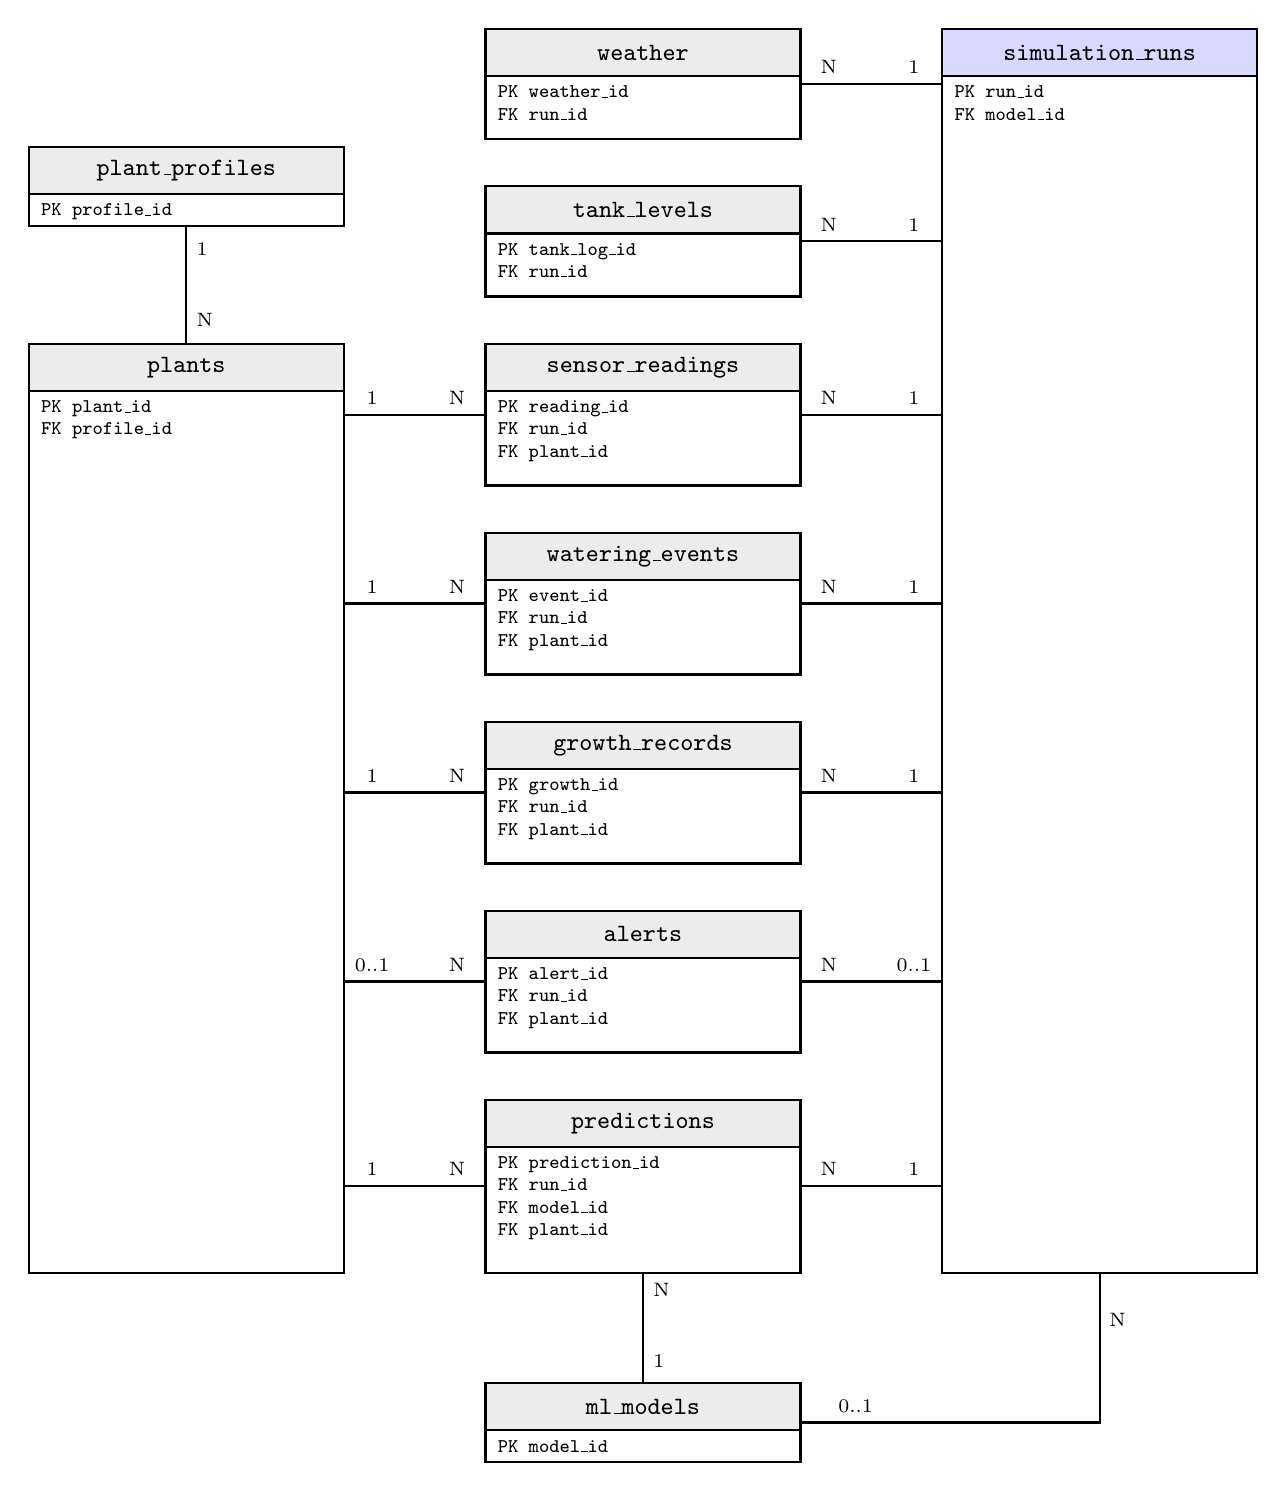
\begin{tikzpicture}[x=1cm,y=1cm]
  % --- relationships (drawn first, boxes on top) ---
  % plant_profiles -> plants
  \draw[thick] (2.0,-2.5) -- (2.0,-4.0)
     node[pos=0.2, right, font=\scriptsize] {1}
     node[pos=0.8, right, font=\scriptsize] {N};
  % plants -> children
  \relh{4.0}{5.8}{-4.9}{1}{N}
  \relh{4.0}{5.8}{-7.3}{1}{N}
  \relh{4.0}{5.8}{-9.7}{1}{N}
  \relh{4.0}{5.8}{-12.1}{0..1}{N}
  \relh{4.0}{5.8}{-14.7}{1}{N}
  % simulation_runs -> children
  \relh{11.6}{9.8}{-0.7}{1}{N}
  \relh{11.6}{9.8}{-2.7}{1}{N}
  \relh{11.6}{9.8}{-4.9}{1}{N}
  \relh{11.6}{9.8}{-7.3}{1}{N}
  \relh{11.6}{9.8}{-9.7}{1}{N}
  \relh{11.6}{9.8}{-12.1}{0..1}{N}
  \relh{11.6}{9.8}{-14.7}{1}{N}
  % ml_models -> predictions
  \draw[thick] (7.8,-17.2) -- (7.8,-15.8)
     node[pos=0.2, right, font=\scriptsize] {1}
     node[pos=0.85, right, font=\scriptsize] {N};
  % ml_models -> simulation_runs (optional)
  \draw[thick] (9.8,-17.7) -| (13.6,-15.8);
  \node[font=\scriptsize, above] at (10.5,-17.7) {0..1};
  \node[font=\scriptsize, right] at (13.6,-16.4) {N};

  % --- entities ---
  \entity{0}{-1.5}{4.0}{1.0}{gray!15}{plant\_profiles}{\textbf{PK} profile\_id}
  \entity{0}{-4.0}{4.0}{11.8}{gray!15}{plants}{\textbf{PK} plant\_id\\\textbf{FK} profile\_id}

  \entity{11.6}{0}{4.0}{15.8}{blue!15}{simulation\_runs}{\textbf{PK} run\_id\\\textbf{FK} model\_id}

  \entity{5.8}{0}{4.0}{1.4}{gray!15}{weather}{\textbf{PK} weather\_id\\\textbf{FK} run\_id}
  \entity{5.8}{-2.0}{4.0}{1.4}{gray!15}{tank\_levels}{\textbf{PK} tank\_log\_id\\\textbf{FK} run\_id}
  \entity{5.8}{-4.0}{4.0}{1.8}{gray!15}{sensor\_readings}{\textbf{PK} reading\_id\\\textbf{FK} run\_id\\\textbf{FK} plant\_id}
  \entity{5.8}{-6.4}{4.0}{1.8}{gray!15}{watering\_events}{\textbf{PK} event\_id\\\textbf{FK} run\_id\\\textbf{FK} plant\_id}
  \entity{5.8}{-8.8}{4.0}{1.8}{gray!15}{growth\_records}{\textbf{PK} growth\_id\\\textbf{FK} run\_id\\\textbf{FK} plant\_id}
  \entity{5.8}{-11.2}{4.0}{1.8}{gray!15}{alerts}{\textbf{PK} alert\_id\\\textbf{FK} run\_id\\\textbf{FK} plant\_id}
  \entity{5.8}{-13.6}{4.0}{2.2}{gray!15}{predictions}{\textbf{PK} prediction\_id\\\textbf{FK} run\_id\\\textbf{FK} model\_id\\\textbf{FK} plant\_id}
  \entity{5.8}{-17.2}{4.0}{1.0}{gray!15}{ml\_models}{\textbf{PK} model\_id}
\end{tikzpicture}
\caption{ER diagram of the waterX database. \textbf{1} = exactly one,
\textbf{N} = many (zero or more), \textbf{0..1} = optional (nullable foreign
key). The line goes from the parent (one) side to the child (many) side.}
\label{fig:er}
\end{figure}

\subsection{Relationships}
All relationships are one-to-many. The schema has no direct one-to-one
relationship. Plants and simulation runs are related many-to-many, which is
resolved through the log tables (\cn{sensor\_readings}, \cn{watering\_events},
\cn{growth\_records}, \cn{predictions}); each carries both a \cn{run\_id} and a
\cn{plant\_id}.

\begin{table}[htbp]
\centering
\small
\begin{tabularx}{\textwidth}{@{}l l l l Y@{}}
  \toprule
  \textbf{Parent (1)} & \textbf{Child (N)} & \textbf{Foreign key} & \textbf{Optional} & \textbf{Meaning}\\
  \midrule
  \cn{plant\_profiles} & \cn{plants} & \cn{profile\_id} & No & A profile defines many plants\\
  \cn{plants} & \cn{sensor\_readings} & \cn{plant\_id} & No & A plant has many readings\\
  \cn{plants} & \cn{watering\_events} & \cn{plant\_id} & No & A plant receives many waterings\\
  \cn{plants} & \cn{growth\_records} & \cn{plant\_id} & No & A plant has many growth records\\
  \cn{plants} & \cn{predictions} & \cn{plant\_id} & No & A plant has many predictions\\
  \cn{plants} & \cn{alerts} & \cn{plant\_id} & Yes & Some alerts (such as low tank) are not tied to a plant\\
  \cn{simulation\_runs} & \cn{weather} & \cn{run\_id} & No & A run contains many weather records\\
  \cn{simulation\_runs} & \cn{sensor\_readings} & \cn{run\_id} & No & A run contains many readings\\
  \cn{simulation\_runs} & \cn{watering\_events} & \cn{run\_id} & No & A run contains many waterings\\
  \cn{simulation\_runs} & \cn{tank\_levels} & \cn{run\_id} & No & A run contains many tank logs\\
  \cn{simulation\_runs} & \cn{growth\_records} & \cn{run\_id} & No & A run contains many growth records\\
  \cn{simulation\_runs} & \cn{predictions} & \cn{run\_id} & No & A run contains many predictions\\
  \cn{simulation\_runs} & \cn{alerts} & \cn{run\_id} & Yes & An alert may be outside any run\\
  \cn{ml\_models} & \cn{simulation\_runs} & \cn{model\_id} & Yes & Only AI-assisted runs use a model\\
  \cn{ml\_models} & \cn{predictions} & \cn{model\_id} & No & A model makes many predictions\\
  \bottomrule
\end{tabularx}
\caption{Foreign-key relationships.}
\end{table}

\subsection{Data Dictionary}

\dbtable{plant\_profiles}{Reusable settings for a plant type, such as basil or tomato.}{
  profile\_id & INTEGER & PK, autoincrement & Unique profile id\\
  name & TEXT & NOT NULL, UNIQUE & Plant type name\\
  min\_moisture & REAL & NOT NULL, 0--100 & Lower moisture limit (\%)\\
  max\_moisture & REAL & NOT NULL, 0--100 & Upper moisture limit (\%); must exceed \cn{min\_moisture}\\
  optimal\_moisture & REAL & NOT NULL & Target moisture (\%)\\
  water\_per\_cycle\_ml & REAL & NOT NULL, $>0$ & Water delivered per watering (ml)\\
  max\_cycles\_per\_day & INTEGER & NOT NULL, default 3 & Safety limit on waterings per day\\
  max\_pump\_seconds & INTEGER & NOT NULL, default 30 & Safety limit on pump run time\\
  schedule\_time & TEXT & nullable & Fixed-schedule time, such as 07:00\\
  uptake\_rate & REAL & NOT NULL & Simulator base water-use rate\\
}

\dbtable{plants}{One plant instance that follows a profile.}{
  plant\_id & INTEGER & PK, autoincrement & Unique plant id\\
  profile\_id & INTEGER & FK to \cn{plant\_profiles}, NOT NULL & The profile this plant follows\\
  name & TEXT & NOT NULL & Plant name\\
  location & TEXT & nullable & Where the plant is\\
  planted\_at & TEXT & NOT NULL & Planting date\\
  active & INTEGER & NOT NULL, default 1 & 1 = active, 0 = deactivated\\
}

\dbtable{simulation\_runs}{One row per simulation run. Same seed with a different strategy gives a fair comparison.}{
  run\_id & INTEGER & PK, autoincrement & Unique run id\\
  strategy & TEXT & NOT NULL, CHECK & \cn{fixed\_schedule}, \cn{rule\_based} or \cn{ai\_assisted}\\
  random\_seed & INTEGER & NOT NULL & Seed for weather and noise\\
  start\_time & TEXT & NOT NULL & Simulation start\\
  end\_time & TEXT & NOT NULL & Simulation end\\
  model\_id & INTEGER & FK to \cn{ml\_models}, nullable & Model used (AI strategy only)\\
  notes & TEXT & nullable & Free text\\
  created\_at & TEXT & NOT NULL, default now & Row creation time\\
}

\dbtable{ml\_models}{Metadata for a prediction method or model; trained-model metrics are optional.}{
  model\_id & INTEGER & PK, autoincrement & Unique model id\\
  name & TEXT & NOT NULL & Model name, such as \cn{random\_forest\_v1}\\
  algorithm & TEXT & NOT NULL & Algorithm used\\
  horizon\_hours & INTEGER & NOT NULL & How many hours ahead it predicts\\
  features & TEXT & NOT NULL & Description or list of input feature names\\
  train\_start, train\_end & TEXT & nullable & Training period\\
  mae, rmse & REAL & nullable & Test-set error metrics\\
  file\_path & TEXT & nullable & Saved model file\\
  created\_at & TEXT & NOT NULL, default now & Row creation time\\
}

\dbtable{weather}{Simulated weather for each run.}{
  weather\_id & INTEGER & PK, autoincrement & Unique id\\
  run\_id & INTEGER & FK to \cn{simulation\_runs}, NOT NULL, cascade delete & Owning run\\
  timestamp & TEXT & NOT NULL & Time of the record\\
  temperature\_c & REAL & nullable & Temperature ($^{\circ}$C)\\
  humidity\_pct & REAL & nullable & Humidity (\%)\\
  sunlight & REAL & nullable & Sunlight level\\
  rain\_mm & REAL & default 0 & Rainfall (mm)\\
  \multicolumn{4}{@{}l}{UNIQUE (\cn{run\_id}, \cn{timestamp})}\\
}

\dbtable{sensor\_readings}{Moisture readings per plant, as the sensor reports them.}{
  reading\_id & INTEGER & PK, autoincrement & Unique id\\
  run\_id & INTEGER & FK, NOT NULL, cascade delete & Owning run\\
  plant\_id & INTEGER & FK to \cn{plants}, NOT NULL & Plant measured\\
  timestamp & TEXT & NOT NULL & Time of the reading\\
  moisture\_pct & REAL & nullable & Noisy sensor value (\%)\\
  true\_moisture & REAL & nullable & Simulator ground truth (NULL on real hardware)\\
  is\_fault & INTEGER & NOT NULL, default 0 & 1 = dropout or spike\\
  \multicolumn{4}{@{}l}{UNIQUE (\cn{run\_id}, \cn{plant\_id}, \cn{timestamp})}\\
}

\dbtable{watering\_events}{Every time the pump waters a plant.}{
  event\_id & INTEGER & PK, autoincrement & Unique id\\
  run\_id & INTEGER & FK, NOT NULL, cascade delete & Owning run\\
  plant\_id & INTEGER & FK, NOT NULL & Plant watered\\
  timestamp & TEXT & NOT NULL & Time of watering\\
  amount\_ml & REAL & NOT NULL, $\geq 0$ & Water delivered (ml)\\
  duration\_s & REAL & nullable & Pump run time (s)\\
  trigger & TEXT & NOT NULL, CHECK & \cn{schedule}, \cn{threshold}, \cn{prediction} or \cn{manual}\\
  moisture\_before & REAL & nullable & Moisture before watering\\
  predicted\_moisture & REAL & nullable & Prediction that triggered it (AI strategy)\\
}

\dbtable{tank\_levels}{Water tank level log.}{
  tank\_log\_id & INTEGER & PK, autoincrement & Unique id\\
  run\_id & INTEGER & FK, NOT NULL, cascade delete & Owning run\\
  timestamp & TEXT & NOT NULL & Time of the log\\
  level\_ml & REAL & NOT NULL & Water left (ml)\\
  capacity\_ml & REAL & NOT NULL & Tank capacity (ml)\\
  \multicolumn{4}{@{}l}{UNIQUE (\cn{run\_id}, \cn{timestamp})}\\
}

\dbtable{growth\_records}{Plant growth over time.}{
  growth\_id & INTEGER & PK, autoincrement & Unique id\\
  run\_id & INTEGER & FK, NOT NULL, cascade delete & Owning run\\
  plant\_id & INTEGER & FK, NOT NULL & Plant measured\\
  timestamp & TEXT & NOT NULL & Time of the record\\
  height\_cm & REAL & nullable & Height (cm)\\
  leaf\_count & INTEGER & nullable & Number of leaves\\
  biomass\_g & REAL & nullable & Biomass (g)\\
  stress\_level & REAL & nullable & 0 (none) to 1 (severe)\\
  \multicolumn{4}{@{}l}{UNIQUE (\cn{run\_id}, \cn{plant\_id}, \cn{timestamp})}\\
}

\dbtable{predictions}{Predicted moisture, stored next to the actual value for evaluation.}{
  prediction\_id & INTEGER & PK, autoincrement & Unique id\\
  run\_id & INTEGER & FK, NOT NULL, cascade delete & Owning run\\
  model\_id & INTEGER & FK to \cn{ml\_models}, NOT NULL & Model that predicted\\
  plant\_id & INTEGER & FK, NOT NULL & Plant predicted\\
  made\_at & TEXT & NOT NULL & When the prediction was made\\
  target\_time & TEXT & NOT NULL & Time being predicted\\
  predicted\_moisture & REAL & NOT NULL & Predicted moisture (\%)\\
  actual\_moisture & REAL & nullable & Filled in later\\
}

\dbtable{alerts}{Warnings raised by the system.}{
  alert\_id & INTEGER & PK, autoincrement & Unique id\\
  run\_id & INTEGER & FK, nullable, cascade delete & Related run\\
  plant\_id & INTEGER & FK, nullable & Related plant\\
  timestamp & TEXT & NOT NULL & Time of the alert\\
  type & TEXT & NOT NULL, CHECK & \cn{low\_tank}, \cn{too\_dry}, \cn{too\_wet}, \cn{sensor\_fault}, \cn{pump\_limit} or \cn{prediction\_dry}\\
  severity & TEXT & NOT NULL, CHECK & \cn{info}, \cn{warning} or \cn{critical}\\
  message & TEXT & nullable & Description\\
  resolved & INTEGER & NOT NULL, default 0 & 1 = resolved\\
}

\subsection{Indexes and Views}
Time-series queries filter by run, plant and time, so these indexes exist:
\begin{itemize}
  \item \cn{sensor\_readings(run\_id, plant\_id, timestamp)}
  \item \cn{watering\_events(run\_id, plant\_id, timestamp)}
  \item \cn{growth\_records(run\_id, plant\_id, timestamp)}
  \item \cn{predictions(run\_id, plant\_id, target\_time)}
  \item \cn{alerts(run\_id, timestamp)}
\end{itemize}
The view \cn{daily\_water\_usage} sums watering-event counts and water use per
run, plant and day. It is available for future reports; the frontend does not
currently query it or provide a strategy-comparison report.

\end{document}
